\chapter{Modellbeschreibung}\label{Modellbeschreibung}
\section{Erzeuger}

Im folgenden wird gezeigt, auf welcher Grundlage die Erzeugungsanlagen in den jeweiligen Inselnetzen modelliert werden. In Anlehnung an den Abschlussbericht des Umweltbundesamtes zur Transformation der Stromerzeugung bis 2050 wird der Fokus ausschließlich auf die Modellierung von Windenergie- und Photovoltaikanlagen gelegt, da diese den Großteil der Erzeugung in allen betrachteten Szenarien darstellen. Zudem bieten sich diese Erzeugungsanlagen besonders für den autarken Einsatz in Inselnetzen an.

\subsection{Wetterdaten}
Die verwendeten Erzeugungsanlagen setzen eine Simulation von Wetterdaten voraus. Für Windenergieanlagen ist daher die Windgeschwindigkeit in $m/s$  und für die Photovoltaikanlagen die Globalstrahlungsdichte in $W/m^2$ von Bedeutung. Diese Daten stellt der deutsche Wetterdienst für über 400 verschiedene Wetterstationen in Deutschland im csv-Dateiformat frei zur Verfügung. Zudem werden die Daten in einer 10-minütigen Auflösung gemessen und bereitgestellt. Für die folgenden Simulationen werden Wetterdaten der anschließend aufgeführten Wetterstionen verwendet.

\begin{center}
	\begin{tabular}[htpb]{c|c|c|c|c}
		Stations ID & Stationshöhe & Länge & Breite & Standort \\
		\hline
		00691 & $4~m$ & 53.0451 & 8.7981 & Bremen \\
		Einschaltgeschwindigkeit & $4~m$ & 54.1860 & 7.9119 & Helgoland Düne
	\end{tabular}
\end{center}

Die Verläufe der Windgeschwindigkeit und Globalstrahlung der beiden Wetterstationen für das Jahr 2022 sind in \autoref{label} zu sehen.

Die Wetterstation in Bremen befindet sich auf freier Fläche in der nähe des Bremer Flughafens und spiegelt daher die Wetterverhältnisse im Umkreis von Bremen wieder. Zur Simulation einer Insel dient die Wetterstation auf Helgoland. Diese zeichnet sich vor allem durch die höhere Windauslastung aus.
\subsection{Windenergie}


Um das Erzeugungsverhalten einer Windenergieanlage zu beschreiben wird im wesentlichen der Zusammenhang zwischen der Windgeschwindigkeit und der ausgegebenen elektrischen Leistung der Anlage benötigt. Als Ansatz hierfür dient die kinetische Energie $E_{kin}$ einer Luftmasse $m$ mit der Geschwindigkeit $v$. \cite{Hau2016}

\begin{equation}
	E_{kin} = \frac{1}{2} mv^3
	\label{eq:wind}
\end{equation}

Im Falle eines Rotors wird eine bestimmte Querschnitsfläche $A$ betrachtet, durch die ein Massenstrom $\dot{m}$ strömt. Dieser lässt sich mithilfe der Luftdichte $\rho$ nach \cite{} wie folgt ausdrücken:

\begin{equation}
	\dot{m} = \rho vA
\end{equation}

Mit Einsetzen in \autoref{eq:wind} ergibt sich somit die enthaltene Leistung im Wind, da die Masse durch den Massenstrom ersetzt wird und sich somit die Energie pro Zeit (Leistung) ergibt.

\begin{equation}
	P_{Wind} = \frac{1}{2}\rho A \nu^3
\end{equation}

%\begin{figure}[H]
%	\centering
%	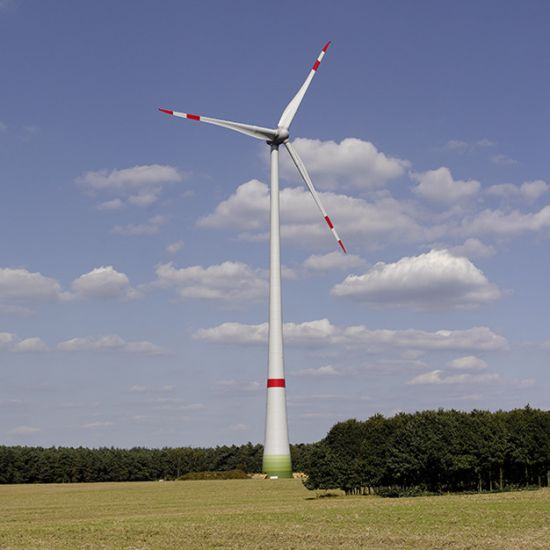
\includegraphics[width=0.7\linewidth]{Abbildungen/E115.jpg}
%	\caption{Enercon E-115}
%	\label{fig:e115}
%\end{figure}
Es zeigt sich, dass die Leistung kubisch von der Windgeschwindigkeit abhängt. Die im Wind enthaltene Leistung wird jedoch nicht vollständig in einer Windenergieanlage in elektrische Leistung umgesetzt. Den Zusammenhang zwischen der Windgeschwindigkeit und der erzeugten Leistung stellt die Leistungskurve einer Anlage dar. Beispielhaft zeigt \autoref{fig:Leistungskurve} die Leistungskurve einer Windenergienalage der Herstellers Enercon. 

\begin{figure}[H]
	\centering
	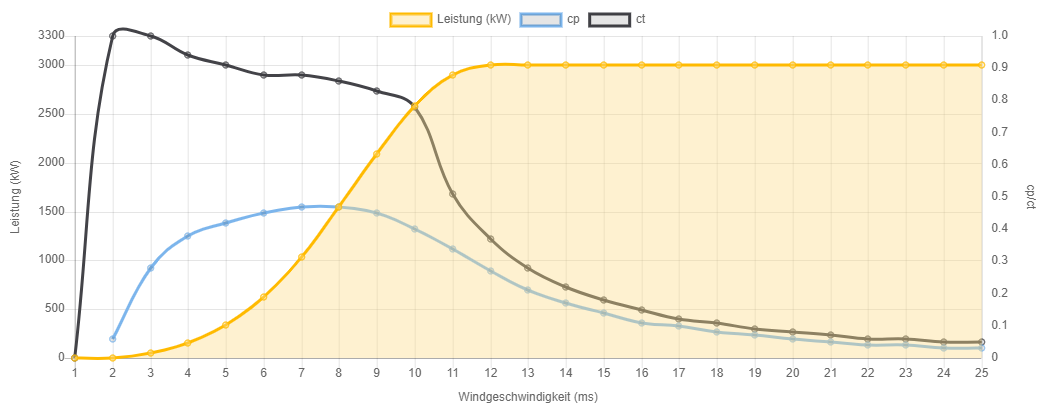
\includegraphics[width=0.9\linewidth]{Abbildungen/Enercon E115.png}
	\caption{Leistungskurve Enercon E-115 \cite{E115}}
	\label{fig:Leistungskurve}
\end{figure}

Dieser Anlagentyp und die zugehörige Leistungskurve dienen auch für die weiteren Simulationen als Datengrundlage. Weitere Parameter, welche für die Simulation relevant sind, werden im folgenden veranschaulicht.

\begin{center}
	\begin{tabular}[htpb]{c|c}
		Typ & Enercon E-115 \\
		\hline
		Nabenhöhe & $149~m$ \\
		Einschaltgeschwindigkeit & $2~m/s$ \\
		Abschaltgeschwindigkeit & $25~m/s$
	\end{tabular}
\end{center}

Wie \autoref{eq:wind} zeigt, ist die erzeugt Leistung stark von der Windgeschwindigkeit abhängig. Diese nimmt wiederum mit steigender Höhe tendenziell zu, weshalb eine Betrachtung der Windgeschwindigkeit in Nabenhöhe notwendig ist. Da die Wetterdaten jedoch meistens in deutlich geringeren Höhen gemessen werden, wird zur Schätzung der Windgeschwindigkeit das logarithmische Windprofil verwendet. Mithilfe von \autoref{eq:log} lässt sich mit der gemessenen Widngeschwindigkeit in einer Höhe unter Angabe der Rauigkeit der Umgebung die Windgeschwindigkeit in einer gewünschten Höhe abschätzen. \cite{Hoehenprofil}

\begin{equation}
	v(h) = \frac{v_{Ref}}{ln\left(\frac{h_{Ref}}{z_0}\right)} \cdot ln\left(\frac{h}{z_0}\right)
	\label{eq:log}
\end{equation}

Mit:

\begin{flushleft}
	\begin{tabular}[htpb]{ll}
		$v(h)$: & Windgeschwindigkeit in Höhe $h$ \\
		$h$: & Höhe über dem Boden \\
		$z_0$: & Bodenrauigkeit \\
		$v_{Ref}$: & Windgeschwindigkeit in Referenzhöhe $h_{Ref}$ 
	\end{tabular}
\end{flushleft}

Bei der Messung in Bodennahen Schichten spielt vorallem die Bodenrauhigkeit eine maßgebliche Rolle, da die Messung hier von der Umgebung stark beeinflußt wird. \autoref{tab:Rauigkeit} zeigt daher die anzunehmenden Werte, je nach Standort der Messstation.  

\begin{table} [H]
	\begin{tabular}[htpb]{p{4cm}|p{3cm}|p{8cm}}
		\textbf{Rauhigkeitsklasse} & \textbf{Rauhigkeitslänge} & \textbf{Geländetyp} \\
		\hline
		0 & 0,0002 & Wasserflächen \\
		\hline
		0,5 & 0,0024 & Offenes Terrain mit glatter Oberfläche, z. B. Beton, Landebahnen auf Flughäfen, gemähtes Gras \\
		\hline
		1 & 0,03 & Offenes landwirtschaftliches Gelände ohne Zäune und Hecken, eventuell mit weitläufig verstreuten Häusern, sehr sanfte Hügel \\
		\hline
		1,5 & 0,055 & Landwirtschaftliches Gelände mit einigen Häusern und 8 Meter hohen Hecken im Abstand von ca. 1.250 Meter \\
		\hline
		2 & 0,1 & Landwirtschaftliches Gelände mit einigen Häusern und 8 Meter hohen Hecken im Abstand von ca. 500 Meter \\
		\hline
		2,5 & 0,2 & Landwirtschaftliches Gelände mit vielen Häusern, Büschen, Pflanzen oder 8 Meter hohen Hecken im Abstand von ca. 250 Meter \\
		\hline
		3 & 0,4 & Dörfer, Kleinstädte, landwirtschaftliche Gebäude mit vielen oder hohen Hecken, Wäldern und sehr raues und unebenes Terrain \\
		\hline
		3,5 & 0,8 & Größere Städte mit hohen Gebäuden \\
		\hline
		4 & 1,6 & Großstädte, hohe Gebäude, Wolkenkratzer \\
	\end{tabular}
\centering
\caption{Angenommene Parameter für die Validierung der Berechnungsmethode \cite{Rauigkeit}}
\label{tab:Rauigkeit}
\end{table}

Die zuvor beschriebenen Zusammenhänge werden nun in einem Simulink Modell verknüpft. Es ergibt sich das Modell in \autoref{fig:simulinkWEA}.

\begin{figure}[H]
	\centering
	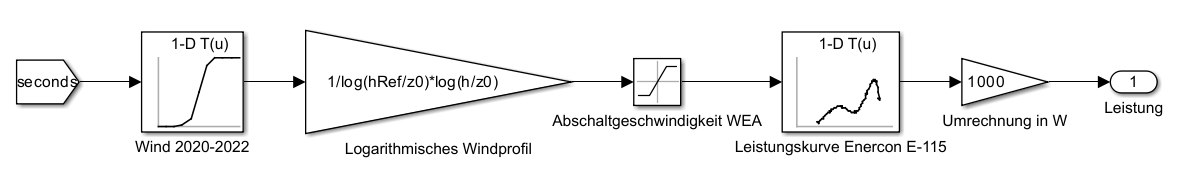
\includegraphics[width=0.9\linewidth]{Abbildungen/ModellWEAeinfach.png}
	\caption{Simulink Modell einer Enercon E-115}
	\label{fig:simulinkWEA}
\end{figure}

Zur Betrachtung des Modells in einem dreiphasigen Netz wird das Modell um einen Dreiphasigen Erzeugerblock ergänzt. Auf eine detaillierte Betrachtung des elektrischen und mechanischen teils der Windenergieanlage wird verzichtet, da dieser für die oberflächliche Betrachtung im Rahmen dieses Projekts keine Rolle spielt. Zudem erhält das Modell zwei PT1-Glieder um die Trägheit der Erzeugung darzustellen. Die Verbindung der Phasen zum Netz über einen Widerstand dient zur Stabilität des Modells während der Simulation.

\begin{figure}[H]
	\centering
	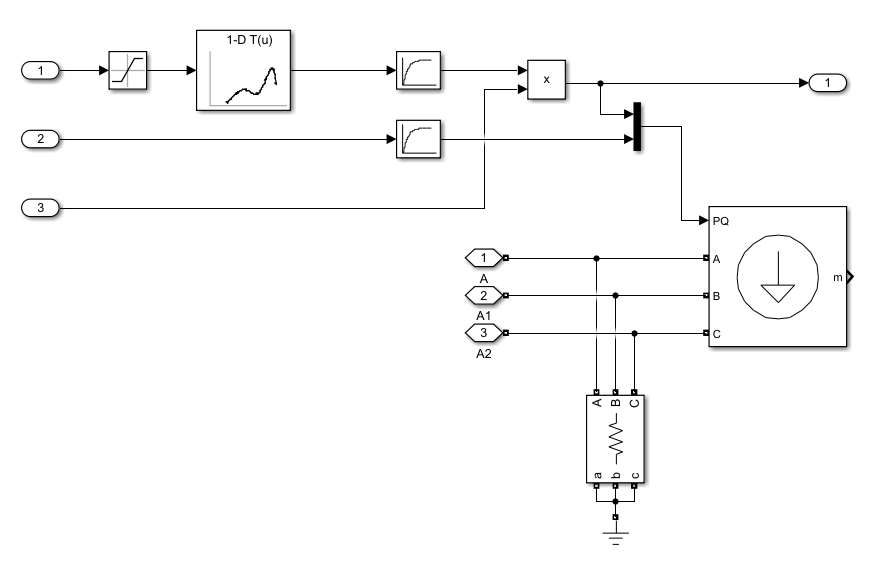
\includegraphics[width=0.9\linewidth]{Abbildungen/ModellWEA.png}
	\caption{Simulink Modell einer Enercon E-115}
	\label{fig:e115}
\end{figure}

\subsection{Photovoltaik}
Ähnlich wie bei der Windenergieanlage wird zur Modellierung einer Photovoltaikanlage ein Bezug zwischen der in der Sonnenstrahlung enthaltenen Energie und der ausgegebenen elektrischen Energie eines PV Moduls hergestellt. Nach \cite{PV} besteht ein proportionaler Zusammenhang zwischen der elektrischen Leistung eines PV-Moduls $P_{el}$ und dem Strahlungsfluss $\Phi$. 

\begin{equation}
	P_{el} = \eta \cdot \Phi
\end{equation}

Der Strahlunfsluss $\Phi$ berechnet sich aus der Starhlungsdichte $E$ und der Fläche $A$. Bei homogener Bestrahlung ergibt sich der folgende Zusammenhang.

\begin{equation}
	\Phi = E \cdot A
\end{equation}

Die Strahlungsdichte $E$ entspricht der gemesenenen Globalstrahlung der betrachtetten Wettestaiuonen.

Die Leistung des Strahlungsflusses wird dabei mit dem Modulwirkungsgrad $\eta$ in elektrische Leistung umgewandelt. Die Verluste sind in \autoref{fig:VerlustePV} in einem Sankey-Diagramm Veranschaulicht. 

\begin{figure}[H]
	\centering
	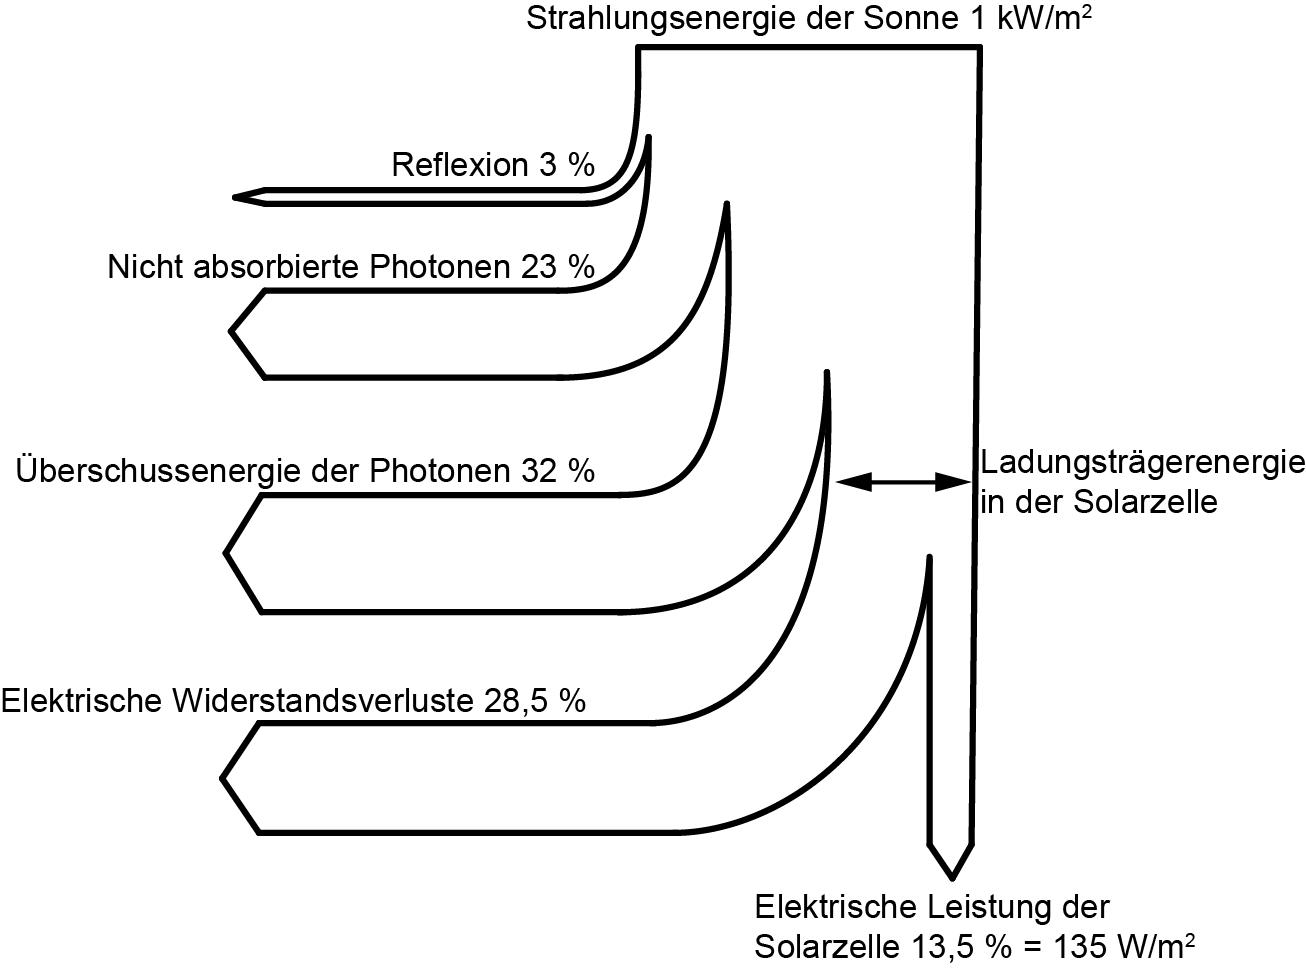
\includegraphics[width=0.7\linewidth]{Abbildungen/WirkungsgradPV.png}
	\caption{Veraqnschaulichung der Verluste innerhalb eines PV-Moduls \cite{VerlustePV}}
	\label{fig:VerlustePV}
\end{figure}

Der hier angegebene Modulwirkunsggrad ist jedoch etwas veraltete und die Wirkungsgrade von Solarmodulen steigen kontinuierlich um etwa 0,3 - 0,5 \%-Punkte pro Jahr, sodass sich aktuell ein Wikrungsgrad von ungefähr 21~\% für kommerzielle Solarmodule ergibt. Im Betrieb wirken sich noch diverse andere nichtlineare Effekte auf den Modulwirkungsgrad aus wie z.B. die Modultemperatur, Verschattung oder die Verschmutzung der Module. Zudem ergeben sich noch zusätzliche Verluste in den Leitungen, Wechselrichtern und Transformatoren der Photovoltaikanlage. Die hier ntstehenden Verluste sind jedoch eher Vernachlässigbar, da beispielsweise Wechselrichter üblicherweise einen Wirkungsrad von 98~\% erreichen. Mit Betrachtung der sonstigen Einflusse auf den Wirkunsgrad wird ein mittlerer Wikrungsgrad von 18~\% zwischen der Strahlungsdichte und der elektrischen Leistung der Anlage angenommen. \cite{FaktenPV} 

Werden die beschriebenen Zusammenhänge in ein Simulink Modell transferiert, ergibt sich das Modell in \autoref{fig:PVModell}

\begin{figure}[H]
	\centering
	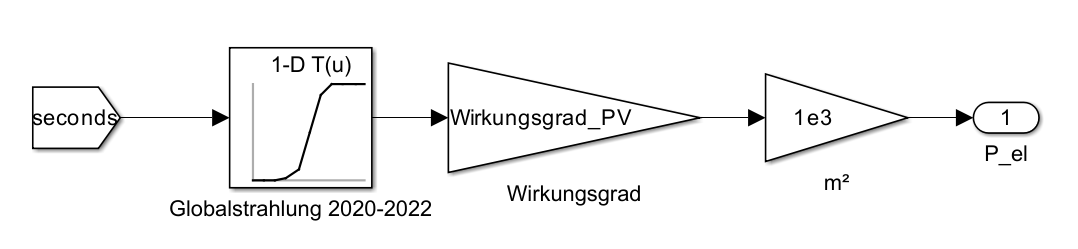
\includegraphics[width=0.9\linewidth]{Abbildungen/PVModell.png}
	\caption{Starkl vereinfachtes Modell einer PV-Anlage in Simulink}
	\label{fig:PVModell}
\end{figure}

Dabei handelt es sich um ein stark vereinfachtes Modell, welches jedoch für diese Betrachtung völlig ausreichend ist, da es die Fluktuation der Sonnenstrahlung wiedergibt.

\section{Verbraucher}
\section{Speicher}\label{Speicher}
In diesem Abschnitt soll der Aufbau und die Steuerung der Speichermodelle erläutert werden.
Dazu werden zunächst verschiedene Batteriemodelle eingeführt und anschließend der gewählte Aufbau für
unsere Simulationen gezeigt. 
Zusätzlich soll die Umsetzung der in Abschnitt~\ref{Betriebsstrategien} angeführten Betriebsstrategien 
beschrieben werden.

\subsection{Batteriemodelle}\label{Batteriemodelle}
Batteriemodelle können grundlegend in 
\begin{itemize}
    \item mathematisch, empirische Black-Box-Modelle,
    \item elektrische Modelle und
   \item physikalisch-chemische Modelle
\end{itemize}
unterteilt werden. 
Innerhalb dieser Kategorien gibt es zusätzlich erhebliche Unterschiede in Bezug auf die Komplexität des Modells.
Die mathematischen Modelle versuchen dabei, das Verhalten von Batterien durch Umsetzung von empirisch bestimmten
Zusammenhängen abzubilden.
So können aus festgelegten Kennparamatern in Verbindung mit Eingangsgrößen die jeweiligen Ausgangsgrößen berechnet werden.
Dabei unterscheiden sich die verschiedenen Modellvarianten stark in ihrer Betrachtung einzelner Aspekte.

In der Kategorie der elektrischen Batteriemodelle wird versucht das Verhalten von Batterien durch Ersatzschaltkreise
mit einfachen elektrischen Bauteilen nachzubilden.
Auch hierbei gibt es große Unterschiede im detailgrad der einzelnen Umsetzungen, es besteht aber die Möglichkeit
auch komplexe elektrochemische Effekte zu modellieren.

Zuletzt bilden die physikalisch-chemischen Modelle wohl die aufwändigste Form.
Durch sie wird versucht auch das Zusammenspiel der einzelnen Materialien innerhalb der Batterie nachzubilden.
Dadurch kann das Verhalten einzelner Batteriezellen sehr genau untersucht werden, in der Praxis sind diese
Modelle aber eher selten zu finden, da die Zusammenhänge auf einer so detaillierten Ebene nur schwer zu ermitteln sind
und Simulationen eher auf das Gesamtverhalten von Batteriesystemen abzielen~\parencite[]{keil2012aufbau}.

Für unsere Simulationen haben wir uns für ein mathematisches Black-Box-Modell entschieden, dass es uns ermöglicht
die Spannung, Leistung und den SOC des Batteriemodells zu betrachten.
Auf Grund der vereinfachten Umsetzung und der insgesamt trotzdem hohen Komplexität des gesamten Simulationsmodells
sollte so die Simulationsdauer möglichst gering gehalten werden.

\begin{figure}[h!]
    \centering
    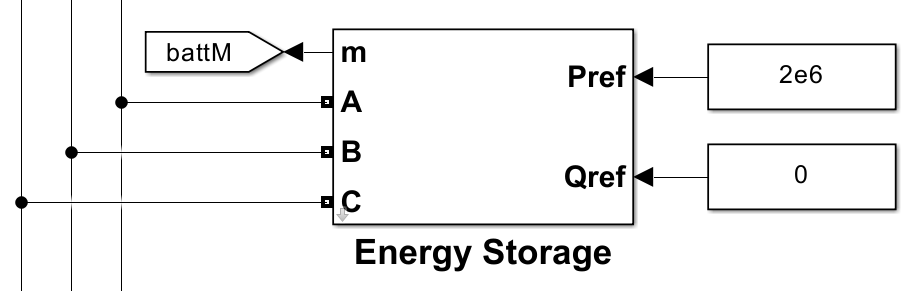
\includegraphics[width=8cm]{Abbildungen/BatterieBlackBox.png}
    \caption{Subsystem-Baustein der Batterie in Simulink}\label{BatModell}
\end{figure}
Abbildung \ref{BatModell} zeigt den Batterie-Block mit den Eingängen zur Wirk- und Blindleistung und den 
Ausgängen für jede Spannungsphase sowie dem Ausgang der Messgrößen.

\begin{figure}[h!]
    \centering
    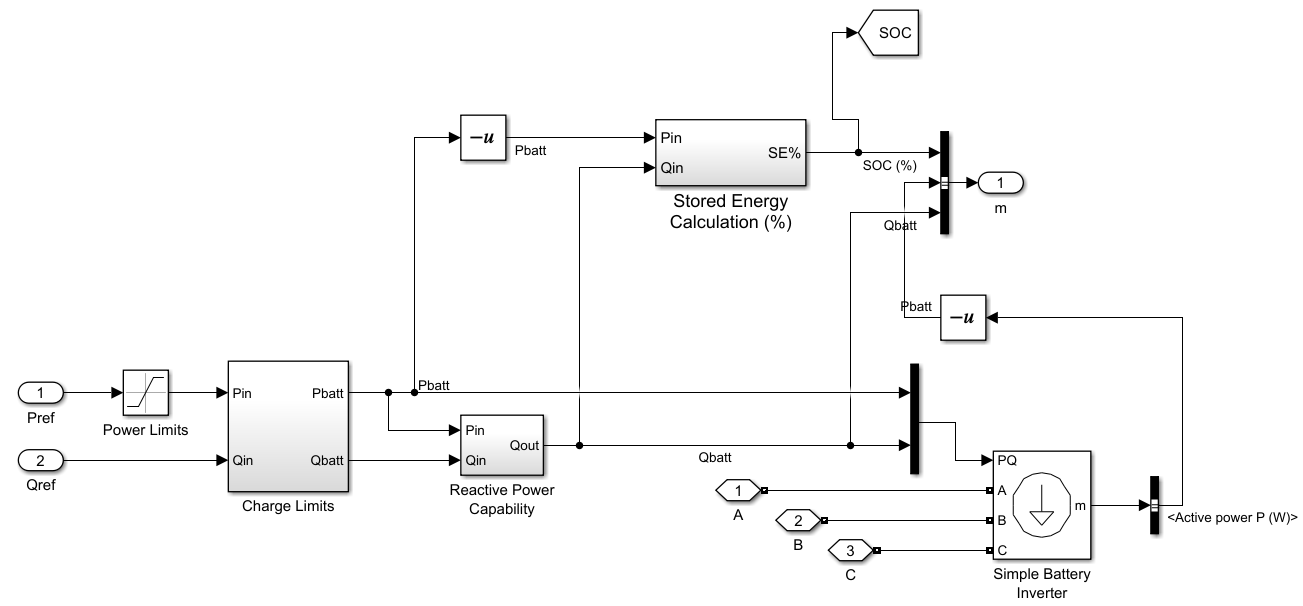
\includegraphics[width=14cm]{Abbildungen/Speicher Ebene1.png}
    \caption{Inhalt des Batteriesubsystems in Simulink}\label{BatModell1}
\end{figure}

Der Aufbau des Subsystems ist in Abbildung~\ref{BatModell1} gezeigt.
Im Wesentlichen besteht das Modell aus einem Block zur Steuerung und Umsetzung der Betriebsstrategien, einem Block
zur Berechnung des SOCs und einer dreiphasigen Last die für dieses Modell als einfacher Umrichter genutzt wird.
Thermische Effekte, Verzögerungen oder Nicht-linearitäten wurden beim Entwurf dieses Modells gänzlich vernachlässigt.
Auch Selbstentladungseffekte oder Aussagen über die Lebensdauer des Batteriespeichers können mit diesem Modell nicht 
betrachtet werden.

Zur Auswertung der Betriebsstrategien und zum groben Entwurf eines realistischen Inselnetzes sollte die Komplexität
des Modells dennoch genügen.
Trotz dieser starken Vereinfachungen laufen Simulationen im dreiphasigen Modell fast in Echtzeit ab.

Während die Steuerung im nächsten Abschnitt~\ref{Lade- und Entlade} genauer erläutert wird soll hier auf die anderen
Komponenten des Batteriemodells etwas näher eingegangen werden.

\paragraph{SOC-Schätzung}
Der Block zur SOC-Schätzung (im Modell als Stored Energy Calculation bezeichnet) basiert auf einem einfachen Leistungsintegral.
Dabei wird aus dem Integral der Batterieleistung die gespeicherte Energiemenge berechnet, welche dann mit der Kapazität der Batterie verglichen wird.
Der SOC zum Zeitpunkt t ergibt sich dann aus
\begin{equation}\label{GL_SOC}
	SOC_{\%}(t) = \frac{E(t)}{C} \cdot 100
\end{equation}
mit
\begin{equation}\label{GL_SOC2}
	E(t) = \int_{0}^{t}p(t) \diff t + E(0) = \int_{0}^{t}p(t) \diff t + \frac{SOC_{\%}(0)}{100}\cdot C.
\end{equation}
Wobei hierbei die korrekte Form der Einheiten zu beachten ist.
Ist die Kapazität der Batterie in $kWh$ gegeben muss das Integral der Leistung entsprechend umgerechnet werden.
Desweitern muss der Momentanwert der Leistung zunächst aus Blind- und Wirkleistung bestimmt werden.
Abbildung~\ref{SOC} zeigt die Umsetzung der beiden Gleichungen~\ref{GL_SOC} und~\ref{GL_SOC2} im Simulink-Modell 
wobei der anfängliche Ladezustand im Integral-Block als Anfangszustand hinterlegt ist.
\begin{figure}[h!]
	\centering
	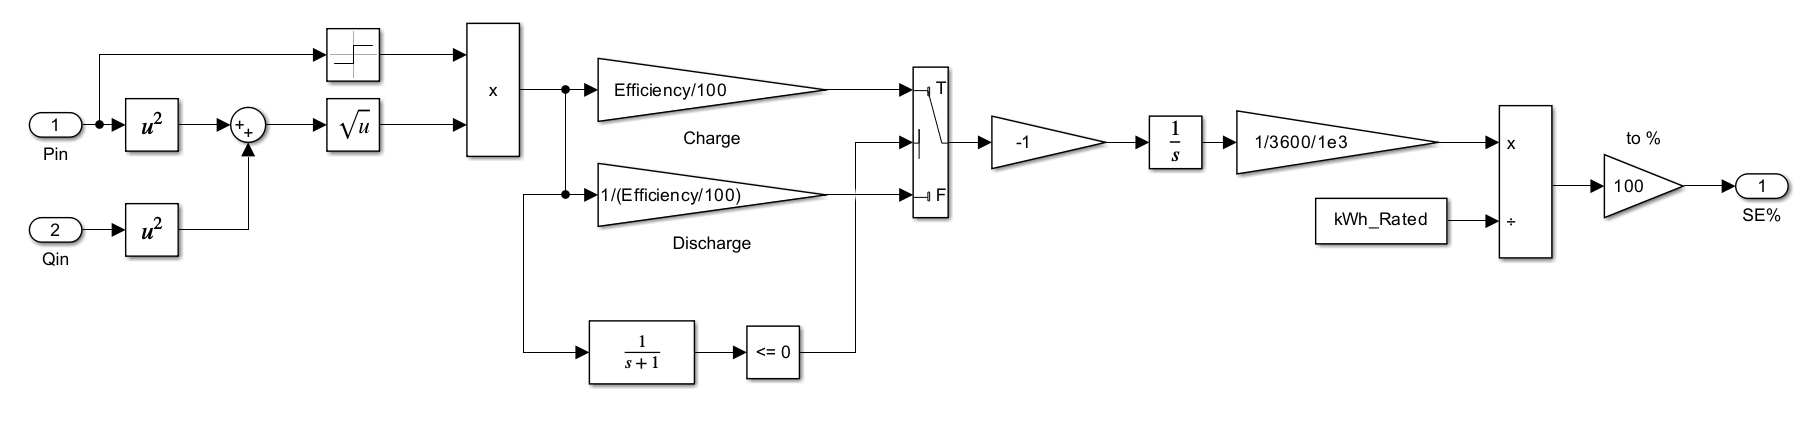
\includegraphics[width=12cm]{Abbildungen/SOC.png}
	\caption{Aufbau der SOC-Schätzung im Simulink Batteriemodell}\label{SOC}
\end{figure}

\paragraph{Dreiphasige Last als Umrichter}
Grundlegend wird in diesem Batteriemodell davon ausgegangen, dass die in der Steuerung festgelegte Leistung
innerhalb der Leistungsgrenzen aber unabhängig vom SOC oder sonstigen Faktoren, exakt an das Netz abgegeben werden kann.
Das ist eine starke aber notwendige Vereinfachung der tatsächlichen Gegebenheiten um überhaupt ein funktionierendes Modell
für diese Projektarbeit zu erstellen.
Durch diese Betrachtung ist es möglich die geforderte Leistung direkt an einen Simulink-Baustein zur dynamischen Last
anzuschließen. 
Ein wesentlicher Vorteil zeigt sich in diesem Baustein, durch die Möglichkeit sowohl negative als auch positive Leistung
an das Netz anzulegen.
Im Block zur Leistungssteuerung wird vorher die Ladeleistung der Batterie als positiv und die Entladeleistung als negativ definiert,
sodass beim Laden der Batterie tatsächlich eine Last am Netz anliegt und beim Entladen bekommt der dynamische Last-Baustein
ein negatives Signal und speist daher Leistung in das Netz ein.

Dieser Block findet seine Anwendung nur in der dreiphasigen Simulation aus Abschnitt~\ref{3phase}.
Da im bilanziellen Modell nur der Leistungsfluss betrachtet wird, braucht es keinen Batterieumrichter.

\subsection{Umsetzung Lade- und Entladestrategien}\label{Lade- und Entlade}
In diesem Abschnitt wird die Umsetzung der in Kapitel~\ref{Betriebsstrategien} beschriebenen Betriebsstrategien erklärt.
Da wir uns entschieden haben, die Batteriespeicher im Inselnetz für die Erbringung von FCR zu nutzen, lag es nahe 
die Deadband-Strategie zu implementieren.
Dafür wurde innerhalb des Simulink-Speicherblocks ein Subsystem erstellt, dass in Abbildung~\ref{Steuerung} zu sehen ist.

\begin{figure}[h!]
	\centering
	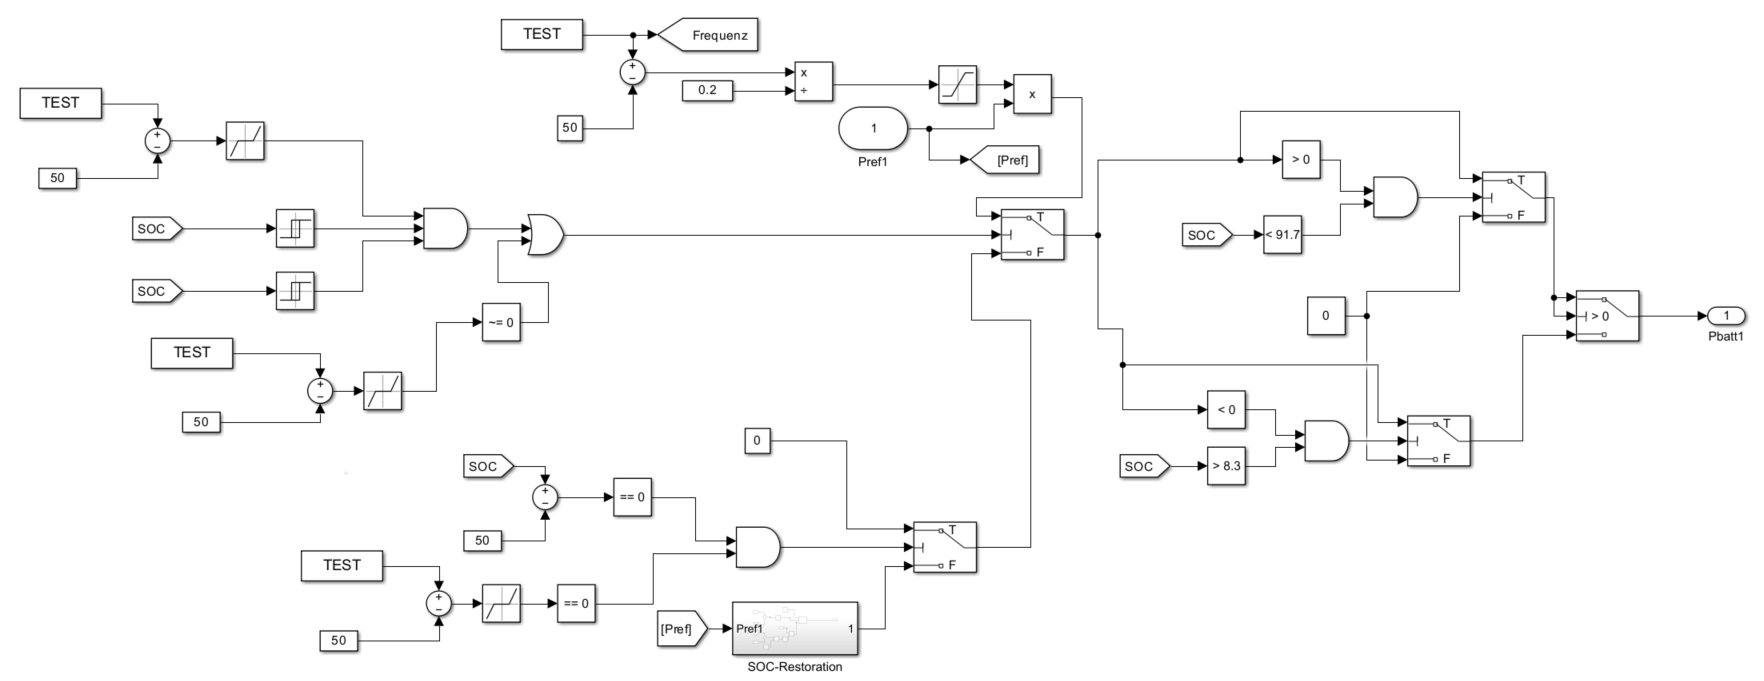
\includegraphics[width=14cm]{Abbildungen/Steuerung.png}
	\caption{Inhalt des Subsystems zur Leistungssteuerung der FCR-Batterie}\label{Steuerung}
\end{figure}

\begin{figure}[h!]
	\centering
	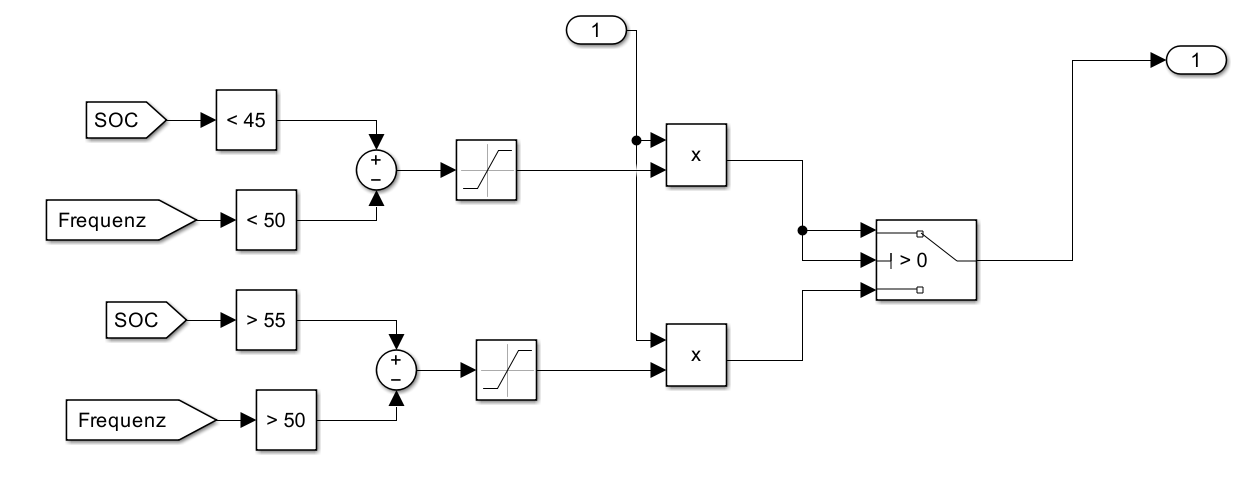
\includegraphics[width=12cm]{Abbildungen/SOC-Rest.png}
	\caption{Inhalt des Steuerblocks zur SOC-Restoration}\label{SOC-Rest}
\end{figure}

\paragraph{Nachweis der Funktion}
Um die Funktion der Batteriesteuerung nachzuweisen wurde eine Simulation mit öffentlichen Frequenzdaten des europäischen Strromnetzes durchgeführt~\parencite[]{noauthor_netztransparenz_nodate}.
Um eine längere Simulation und Auswertung zu ermöglichen wurde das Batteriemodell vom Rest des Inselnetzes isoliert betrachtet.
Während der Simulation mit den sekündlichen Frequenzwerten wurde der SOC und die Leistung der Batterie aufgezeichnet.



\section{Netzmodell}
\subsection{Bilanziell}
\subsection{Dreiphasig}\label{3phase}


\chapter{Simulationsergebnisse}

\chapter{Auswertung}
